\section{Introduction} \label{sec:intro}



\section{The Faro Framework} \label{sec:faro}

\faro has adopted a modular and extensible design that can be configured  to run any subset of metrics on any subset of data products, e.g., a  subset of the realtime metrics computed on a single exposure. 
Two main components form the basis of the \faro framework;  a collection of \texttt{Task}s that compute specific metric values, and a set of base classes that handle data i/o for various types of input data units corresponding to the granularity of metric computation, e.g., per-detector, per-visit, per-patch, per-tract. 
\faro builds upon much of the existing infrastructure of the LSST Science Pipelines, in particular the ``Generation 3'' middleware, including the Data Butler and Task Framework\footnote{\url{https://pipelines.lsst.io/modules/lsst.pipe.base/task-framework-overview.html}}\cite{dmtn-229}, and the LSST verification framework\cite{SQR-019}. 
The LSST Data Butler (hereafter the ``Butler'') provides an abstracted data access interface that is used to read and write data without having to know the details of file formats or locations.
The Butler organizes data, both raw and processed, into data repositories.
A \texttt{Task} is a reusable unit of code in the LSST science pipelines infrastructure that is used to process data.
Each Task has a specialized configuration object attached to it and provides a \texttt{run()} method that implements the algorithm to execute. 
Each \faro metric has an associated \texttt{Task} class that implements the mathematical algorithm to compute the scalar metric value on the input data.
The LSST Verification Framework, \texttt{lsst.verify}, is a framework for making verification measurements in the LSST Science Pipelines.
\faro takes as input catalog data products generated by the LSST Science Pipelines\footnote{The LSST science pipelines produce catalog data products both in FITS and parquet file format. \faro works exclusively with with parquet formatted data.} stored in a Butler repository, 
%  but in principle could use any data product available in a Butler repository, including images, 
 and computes scalar performance metrics on them. 
The resulting metric values
% \footnote{The result of computing a given metric on some set dataset.} 
are persisted in the same Butler repository alongside the input data products, each with an associated searchable data identifier\footnote{A dict-like identifier for data usable across multiple Butler collections and DatasetTypes.} as \texttt{lsst.verify.Measurement} objects.

\subsection{Analysis Contexts} \label{ssec:contexts}

An analysis context defines the type of input data unit corresponding to the granularity of metric computation, e.g per-detector, per-visit, per-patch or per-tract.
\faro supports metric calculation for a multiple analysis contexts, that is, the same mathematical function can be called in a different analysis context to produce a different metric value. 
For example, the residual PSF ellipticity correlation metrics can be computed on a per-visit or per-tract analysis context. 
For some metrics, only certain analysis contexts make sense and often the choice of analysis context will be dictated by statistics, e.g a small 1\degsq CI dataset may not contain enough data to compute some metrics on a per-tract level. 
\faro allows users to easily define a new analysis contexts for their particular science need. 

The following analysis, corresponding to analysis contexts  are currently supported in \faro:
\begin{itemize}
\item per-detector source catalogs i.e., single-visit detections
\item per-visit source catalogs i.e., single-visit detections
\item per-patch object catalogs i.e., coadd detections both per-band and multi-band
\item per-tract object catalogs i.e., coadd detections, both per-band and multi-band input
\item per-patch matched source catalogs, i.e., set of single-visit detections of the same objects, both single band and multi-band input
\item per-tract matched source catalogs, i.e., set of single-visit detections of the same objects 
\end{itemize}

\subsection{Base Classes} \label{ssec:baseclasses}

\faro provides a set of base classes corresponding to the various analysis contexts described above that use the \texttt{PipelineTask} framework to build a quantum graph\footnote{A data structure that represents a concrete workflow generated from a Pipeline.} and interact with Butler for data i/o.
The base classes abstract away the data i/o, leaving the scientist free to focus on the algorithmic details  relevant to their particular analysis. 
The primary base classes in the lsst.faro package are \texttt{CatalogMeasurementBaseConnections}, to define the desired i/o,  \texttt{CatalogMeasurementBaseConfig}, to provide the configuration, and \texttt{CatalogMeasurementBaseTask}, to run the algorithm and store teh output data in the Butler. 
Each of these base classes inherits from \texttt{MetricConnections}, \texttt{MetricConfig}, and \texttt{MetricTask}, in the \texttt{lsst.verify} package respectively, and adds additional general functionality for computing science performance metrics based on Source and Object catalog inputs. 
Additional base classes can be easily added following this scheme for new analysis contexts. 

\subsection{Stages of Metric Computation} \label{ssec:stages}

Metric computation with \faro proceeds through three stages:
\begin{enumerate}
\item \textbf{Preparation:}  any intermediate data products that are needed as input to the subsequent measurement step are assembled and persisted in the Butler.	
\item \textbf{Measurement:} the metric \texttt{Task} is run to compute a measurement for each unit of data (i.e., a quantum of processing with a particular a dataId for the output measurement). Measurements are stored as \texttt{lsst.verify.Measurement} objects.
\item \textbf{Summary:}  a single scalar summary statistic, e.g a mean, median, etc is generated from the collection of input measurements computed in the measurement stage.  Summary statistics are stored as \texttt{lsst.verify.Measurement} objects and persisted in the Butler.
\end{enumerate}
Not all metrics will necessarily have a  preparation stage as there may be no additional intermediate data products needed to compute the metric than those generated as part of the pipelines processing, however all must have a measurement and summary stage. 

Take as an example the photometric repeatability metric, PA1, which measures the RMS photometric repeatability of bright non-saturated unresolved point sources in a single filter.
During the preparation stage, a matched source catalog is created for each tract and band that matches source detections in individual visits that correspond to the same physical astronomical object\footnote{LSST defines an Object as an astrophysical physical object, e.g a star, galaxy or asteroid, and a Source as a  single detection of an astrophysical object in an image. The association of Sources that are non-moving lead to Objects; the association of moving Sources leads to Solar System Objects.}. 
During the measurement stage, for each tract and band, the matched catalog computed and stored in the preparation stage is loaded into memory and used to compute the RMS scatter of fluxes for a single astrophysical object. 
In the final summary stage, the measurements for the ensemble of individual tracts computed in the measurement stage are loaded to compute a median summary statistic per band. 
This final summary statistic characterizes the overall performance for the dataset per band and is stored as an \texttt{lsst.verify} object in the Butler. 

\subsection{Processing Pipelines} \label{ssec:pipelines}


Pipelines, configurations in the form of YAML files, are used to define the \faro metrics to be computed together with the  detailed execution parameters for metric calculations. 
The \faro package provides a set of pre-defined pipelines, defined per analysis context, for many common configurations of computing metrics. 
\faro pipelines can be run as an after burner to the LSST Science Pipelines or can be interspersed with science pipelines processing to compute , as long as the necessary input data products have been computed and are stored in the Butler.  
For example, all single-visit metrics can already be computed once the single-frame processing steps have completed. 
This enables us to promptly assess performance and take any corrective action early. 
Figure \ref{fig:faro_pipeline} shows an example of a \faro pipeline describing the measurement stage of the computation of three performance metrics  using a per-tract matched catalog analysis context.
Pipelines can be built hierarchically, with a high-level pipeline calling lower-level pipelines, as shown in figure \ref{fig:faro_pipeline_hierarchy}.

\begin{figure}[h]
  \lstset{language=YAML}
  \begin{lstlisting}
description: Compute metrics from matched catalogs
tasks:
  PA1:
    class: lsst.faro.measurement.TractMatchedMeasurementTask
    config:
      connections.package: validate_drp
      connections.metric: PA1
      python: |
        from lsst.faro.measurement import PA1Task
        config.measure.retarget(PA1Task)
  PF1_design:
    class: lsst.faro.measurement.TractMatchedMeasurementTask
    config:
      connections.package: validate_drp
      connections.metric: PF1_design_gri
      python: |
        from lsst.faro.measurement import PF1Task
        config.measure.retarget(PF1Task)
        config.measure.threshPA2 = 15.0
  AM1:
    class: lsst.faro.measurement.TractMatchedMeasurementTask
    config:
      connections.package: validate_drp
      connections.metric: AM1
      python: |
        config.connections.matchedCatalog = 'matchedCatalogTractMag17to21p5'
        from lsst.faro.measurement import AMxTask
        config.measure.retarget(AMxTask)
        config.measure.annulus_r = 5.0
    \end{lstlisting}
  \caption{A \faro pipeline describing the measurement stage of the computation of three performance metrics per-tract from matched catalogs.}
  \label{fig:faro_pipeline}
\end{figure}

\begin{figure}[h]
  \lstset{language=YAML}
  \begin{lstlisting}
description: Complete metrics measurement pipeline
imports:
  # Photometric and astrometric repeatability:
  - location: $FARO_DIR/pipelines/metrics_pipeline_matched.yaml
  # Astrometry relative to a reference band:
  - location: $FARO_DIR/pipelines/metrics_pipeline_matched_multi.yaml
  # Ellipticity residual correlations, visit-level:
  - location: $FARO_DIR/pipelines/metrics_pipeline_visit.yaml
  # Ellipticity residual correlations, coadds:
  - location: $FARO_DIR/pipelines/metrics_pipeline_tract.yaml
  # Stellar locus width:
  - location: $FARO_DIR/pipelines/metrics_pipeline_tract_multi.yaml
    \end{lstlisting}
  \caption{A  \faro pipeline showing how pipelines for pre-defined groups of metrics, repeatability metrics or visit-level metrics can be called hierarchically.}
  \label{fig:faro_pipeline_hierarchy}
\end{figure}

\section{Adding a  Metric} \label{sec:add}

We anticipate that many developers and scientists will want to define write their own metrics specifically to address concerns that arise as LSST progresses through the construction phase and into operations.
The first step in writing a new metric is to define the analysis context (\S \ref{ssec:analysis_context}) and to review the associated \texttt{Connections},  \texttt{Config}, and  \texttt{Task} base classes (\S \ref{ssec:base_classes}) to understand the in-memory python objects that will be passed to the run method of the metric measurement task, and the configuration options.
If the required analysis context and associated base class do not exist, they must first be created. 
Once the analysis context and base class are defined, the metric can be implemented by creating a measurement \texttt{Task}, an instance of \texttt{lsst.pipe.base.Task} that will operate on in-memory python objects and compute the metric. 
Finally, the new metric is added to the appropriate pipeline YAML file so that it can be run.
Figures \ref{fig:num_sources_task} show an example of a non-normative metric \texttt{Task} written to compute the number of rows in an input Source or Object catalog, \texttt{NumSourcesTask}

\begin{figure}[htb]
  \lstset{language=python}
  \begin{lstlisting}
  
class NumSourcesTask(Task):
    r"""Simple default task to count the number of sources/objects in catalog."""

    ConfigClass = NumSourcesConfig
    _DefaultName = "numSourcesTask"

    def run(self, metricName, catalog, **kwargs):
        """Run NumSourcesTask
        Parameters
        ----------
        metricName : `str`
            The name of the metric to measure.
        catalog : `dict`
            `lsst.afw.table` Catalog type
        kwargs
            Extra keyword arguments used to construct the task.
        Returns
        -------
        measurement : `Struct`
            The measured value of the metric.
        """
        self.log.info("Measuring %s", metricName)
        if self.config.doPrimary:
            nSources = np.sum(catalog[self.config._getColumnName(
                "detect_isPrimary")] is True)
        else:
            nSources = len(catalog)
        self.log.info("Number of sources (nSources) = %i" % nSources)
        meas = Measurement("nsrcMeas", nSources * u.count)
        return Struct(measurement=meas)    \end{lstlisting}
        
  \caption{Implementation of NumSourcesTask, a metric to compute the number of sources in an input catalog. }
  \label{fig:num_sources_task}
  \par\medskip
\end{figure}

\section{Tracking and Visualization} \label{sec:tracking}


\section{Faro Applications} \label{sec:applications}

\subsection{Monitoring Science Pipelines Performance} \label{ssec:monitoring}

\subsubsection{Precursor datasets} \label{sssec:datasets}

\subsubsection{Continuous Integration}\label{sssec:ci}

\subsubsection{Software Release Characterization } \label{sssec:characterization}


\begin{figure}[htb]
  \centering
  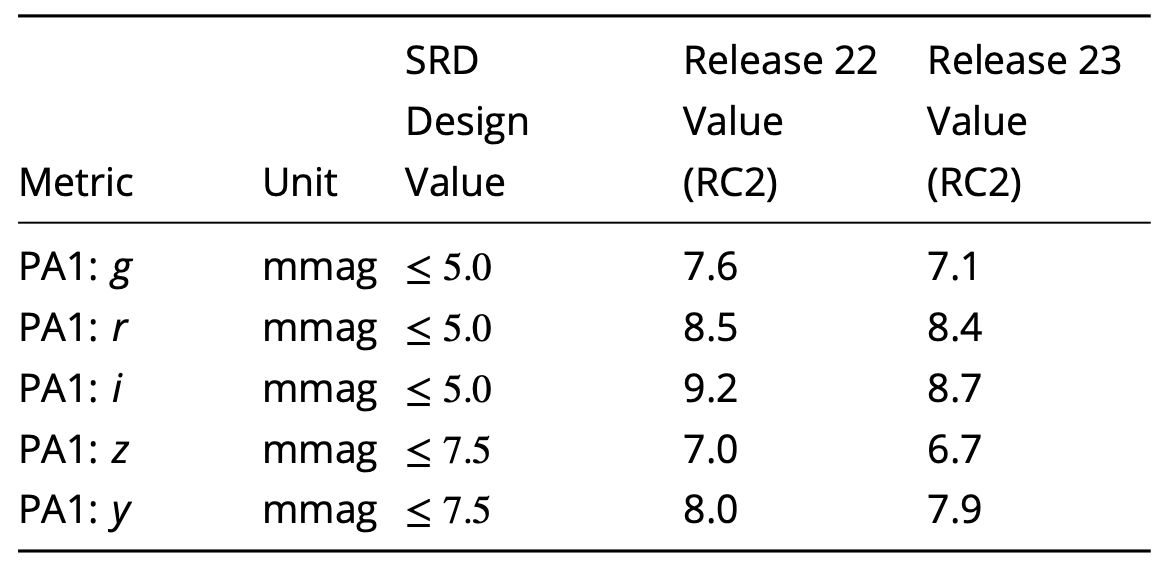
\includegraphics[width=0.45\textwidth]{figures/cmr_r23_photometric_metrics} 
  \hspace{0.5cm}
  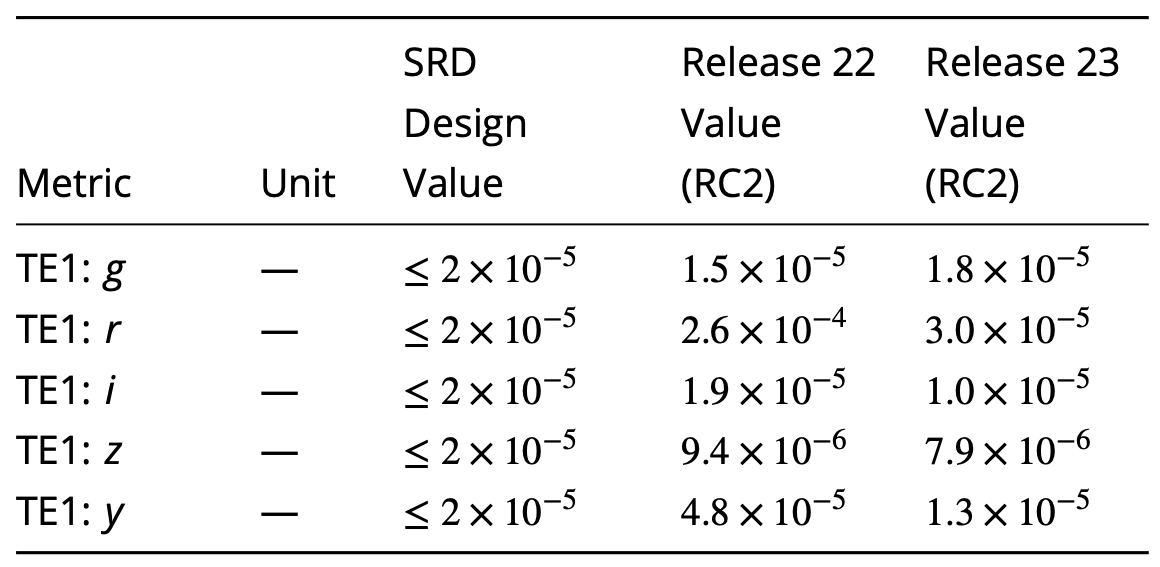
\includegraphics[width=0.45\textwidth]{figures/cmr_r23_ellipticity_metrics}
  \par\medskip % force a bit of vertical whitespace
  \caption{Excerpt from the  LSST Science Pipelines major Release 23 Characterization Metric Report on the HSC RC2 dataset. Metric values are compared with those of the previous release of the science pipelines and with the  design values from the LSST Science Requirements document SRD.}
  \label{fig:cmr_r23}
\end{figure}

\subsection{Rubin Auxiliary Telescope} \label{ssec:auxtel}

\subsection{Rubin Data Previews} \label{ssec:datapreviews}

\section{Current Status and Future Development} \label{sec:future}

\section{Conclusions} \label{sec:conclusions}